
\begin{figure}[t]
    \centering
    % \vspace{-0.5em}
    \setlength{\tabcolsep}{0pt}
    \newcommand\figwidth{.24}
    % \renewcommand{\arraystretch}{1.5}
    \begin{subfigure}{0.55\linewidth}
        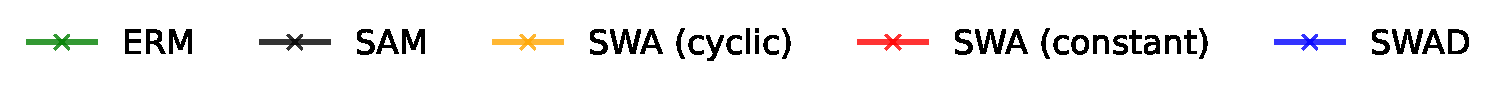
\includegraphics[width=\linewidth]{figures/flatness/legend.pdf}
    \end{subfigure}\\
    %
    % \begin{subfigure}{1.0\linewidth}
        \centering
        \begin{subfigure}{0.3\linewidth}
            \setlength{\abovecaptionskip}{3pt}
            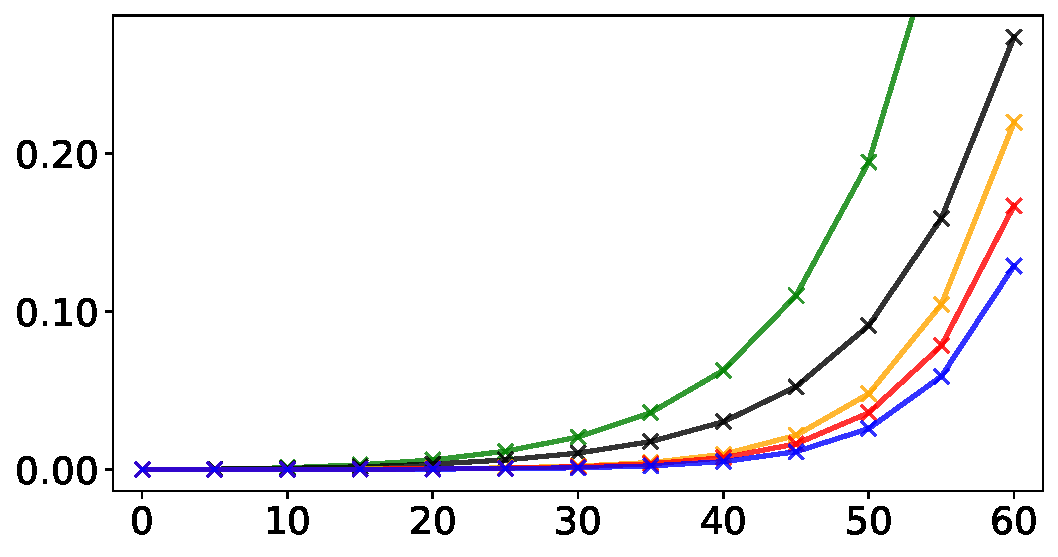
\includegraphics[width=\linewidth]{figures/flatness/PACS_TE4_Train_S5_MD60_N100_BNFalse.pdf}
            \caption{Average train flatness}
        \end{subfigure}
        \quad
        \begin{subfigure}{0.3\linewidth}
            \setlength{\abovecaptionskip}{3pt}
            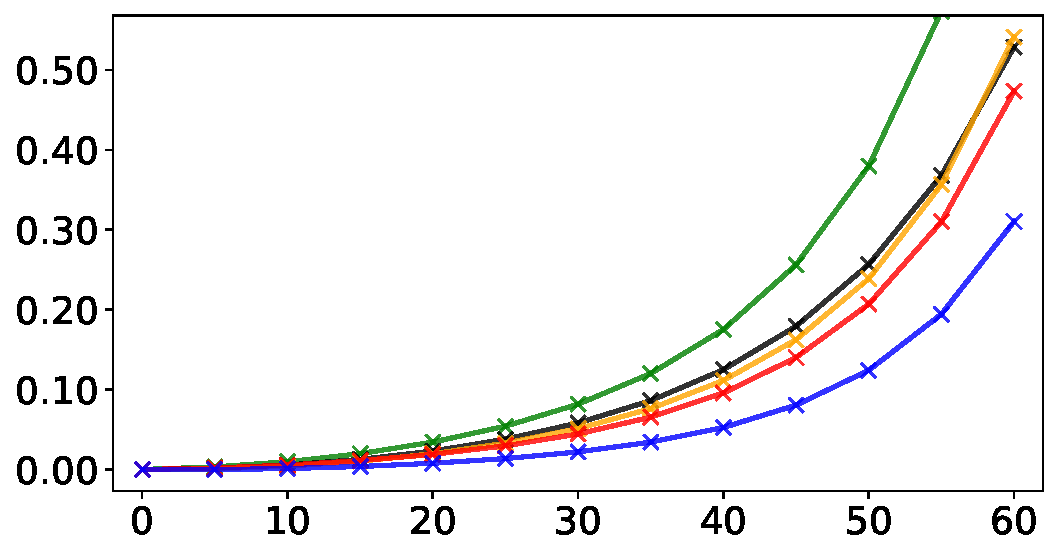
\includegraphics[width=\linewidth]{figures/flatness/PACS_TE4_Test_S5_MD60_N100_BNFalse.pdf}
            \caption{Average test flatness}
        \end{subfigure}
    %     \caption{\small Averaged flatness on \data{PACS} dataset. Left and right figures indicate averaged train and test flatness, respectively.}
    % \end{subfigure}
    \\\vspace{0.4em}
    \begin{subfigure}{1.0\linewidth}
        \begin{tabular*}{\textwidth}{c @{\extracolsep{\fill}} cccc}
            \rotatebox[origin=c]{90}{Train}
            &
            \raisebox{-0.45\height}{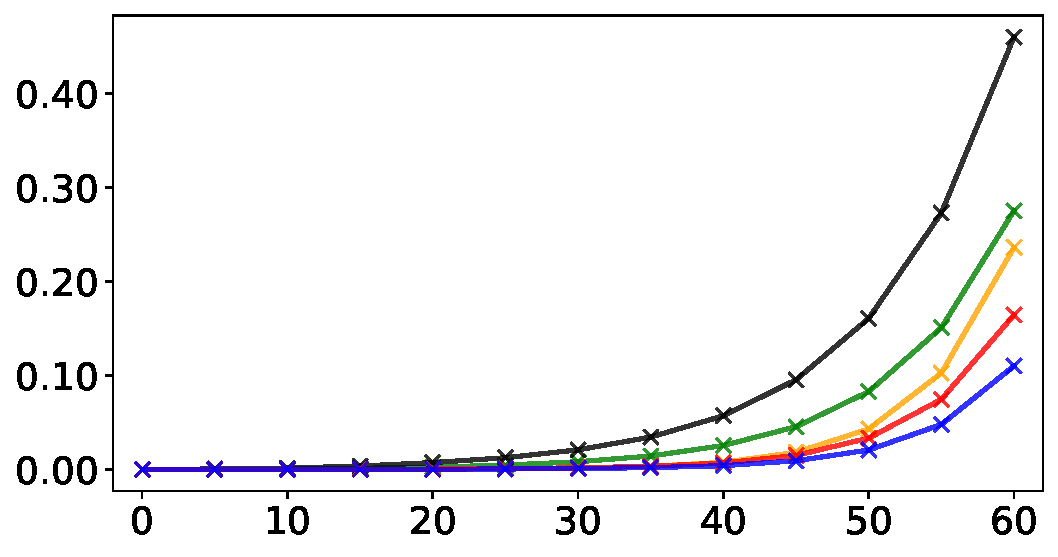
\includegraphics[width=\figwidth\textwidth]{figures/flatness/PACS_TE0_Train_S5_MD60_N100_BNFalse.pdf}}
            &
            \raisebox{-0.45\height}{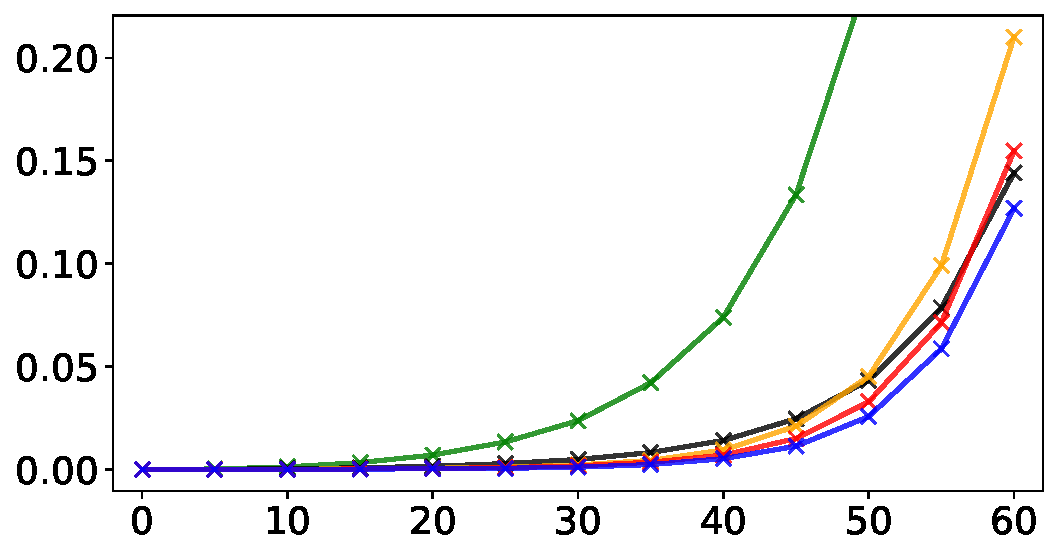
\includegraphics[width=\figwidth\textwidth]{figures/flatness/PACS_TE1_Train_S5_MD60_N100_BNFalse.pdf}}
            &
            \raisebox{-0.45\height}{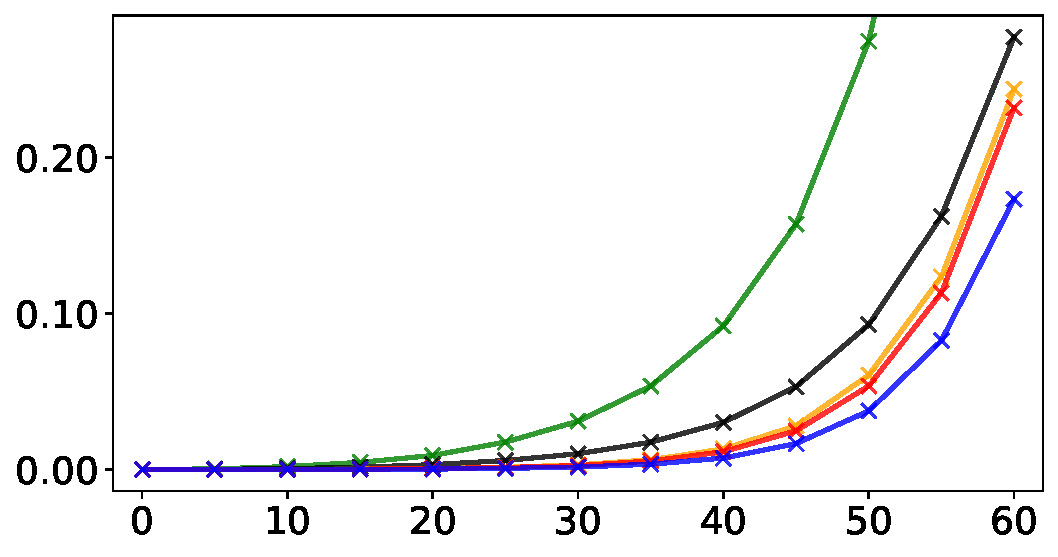
\includegraphics[width=\figwidth\textwidth]{figures/flatness/PACS_TE2_Train_S5_MD60_N100_BNFalse.pdf}}
            &
            \raisebox{-0.45\height}{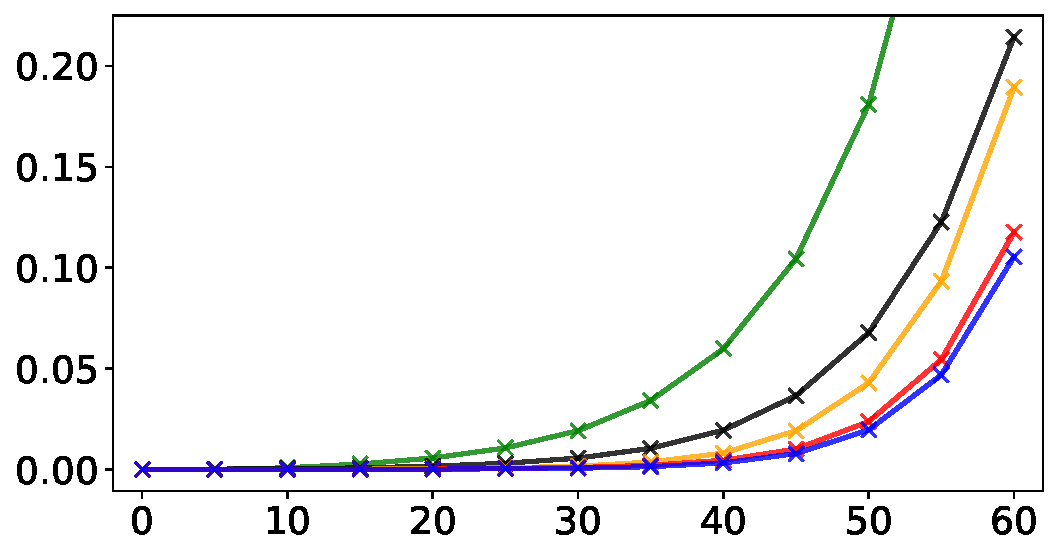
\includegraphics[width=\figwidth\textwidth]{figures/flatness/PACS_TE3_Train_S5_MD60_N100_BNFalse.pdf}}
        \\
            \rotatebox[origin=c]{90}{Test}
            &
            \raisebox{-0.5\height}{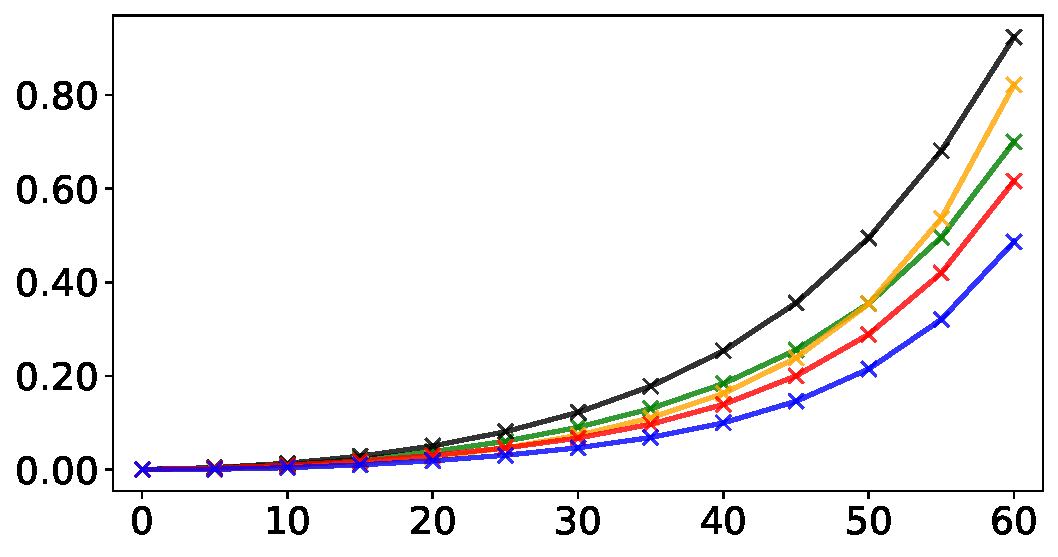
\includegraphics[width=\figwidth\textwidth]{figures/flatness/PACS_TE0_Test_S5_MD60_N100_BNFalse.pdf}}
            &
            \raisebox{-0.5\height}{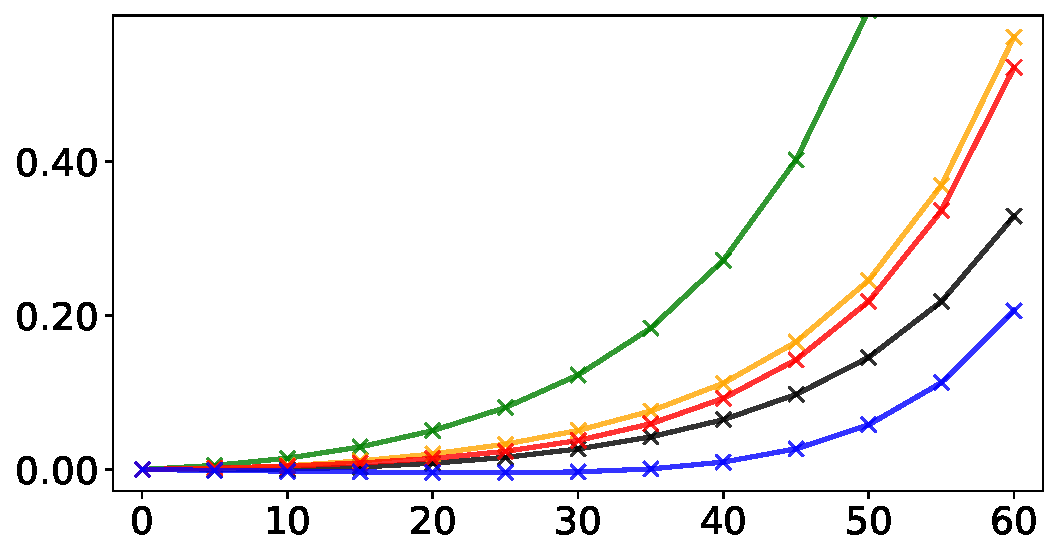
\includegraphics[width=\figwidth\textwidth]{figures/flatness/PACS_TE1_Test_S5_MD60_N100_BNFalse.pdf}}
            &
            \raisebox{-0.5\height}{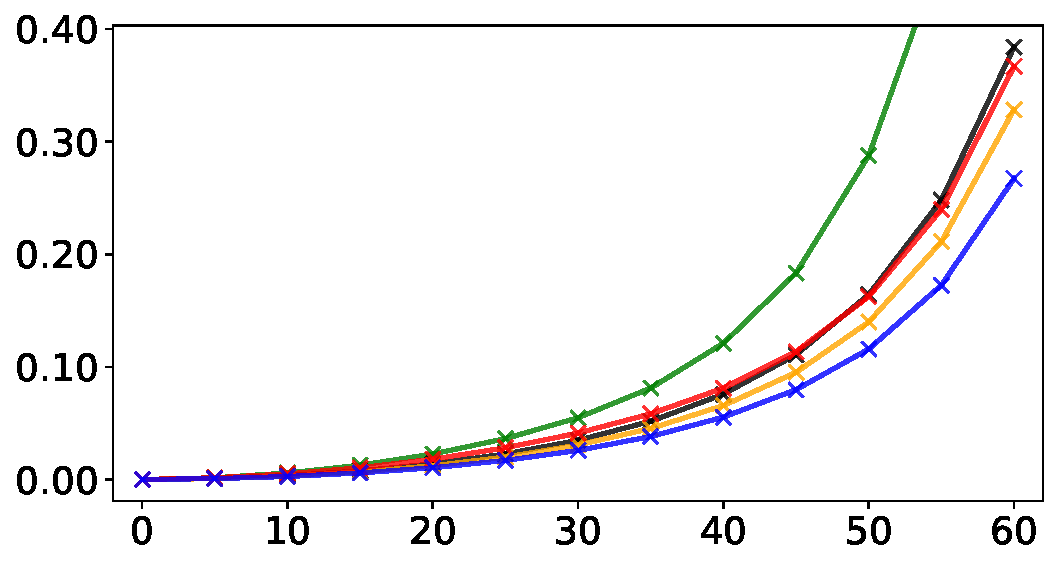
\includegraphics[width=\figwidth\textwidth]{figures/flatness/PACS_TE2_Test_S5_MD60_N100_BNFalse.pdf}}
            &
            \raisebox{-0.5\height}{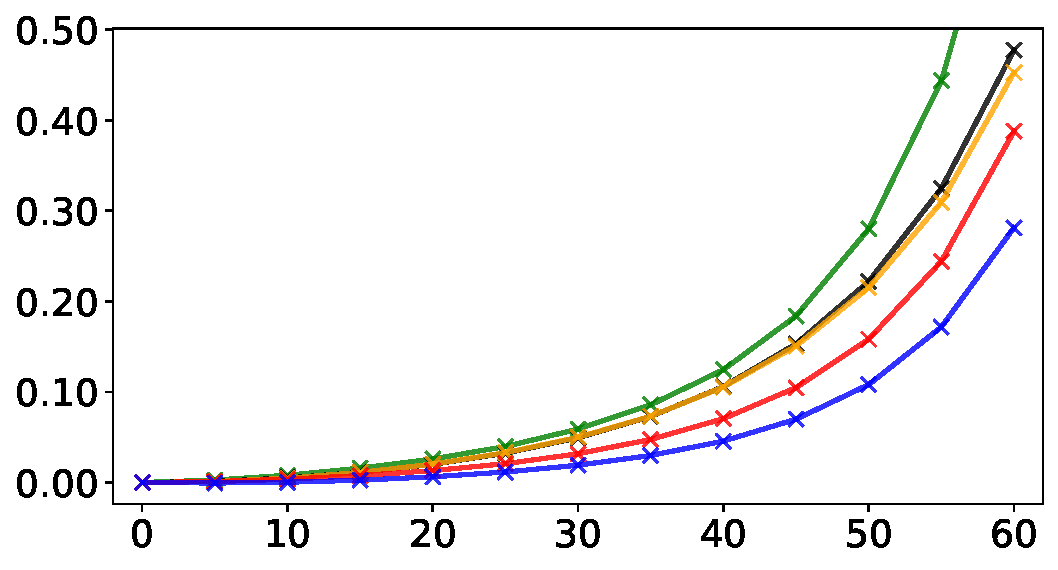
\includegraphics[width=\figwidth\textwidth]{figures/flatness/PACS_TE3_Test_S5_MD60_N100_BNFalse.pdf}}
        \\
            &
            {\small \textit{Art painting} (test)}
            &
            {\small \textit{Cartoon} (test)}
            &
            {\small \textit{Photo} (test)}
            &
            {\small \textit{Sketch} (test)}
        \end{tabular*}
        \setlength{\abovecaptionskip}{3pt}
        \caption{\small Flatness for each target domain}
    \end{subfigure}
    \caption{\small \textbf{Local flatness comparisons.} We plot the local flatness via loss gap, \ie, $\mathcal{F}_\gamma(\theta)=\mathbb {E}_{\| \theta' \| = \|\theta\| + \gamma} [\mathcal{E}(\theta')-\mathcal{E}(\theta)]$, of ERM, SAM, SWA, and SWAD by varying radius $\gamma$ on different domains of \data{PACS} dataset. For each figure, Y-axis indicates the flatness $\mathcal{F}_\gamma(\theta)$ and X-axis indicates the radius $\gamma$. We measure the train flatness $\mathcal{F_\gamma^D}(\theta)$ on seen domains and the test flatness $\mathcal{F_\gamma^T}(\theta)$ on unseen domain. Each point is computed by Monte-Carlo approximation with 100 random samples. This comparisons show SWAD finds flatter minima than not only ERM but also SAM and SWA.
    %, in both train and test domains.
    }
    \label{fig:flatness}
\vspace{-1em}
\end{figure}
